\section{Третья программа}
\subsection{Базовый вариант}
\begin{code}
	\captionof{listing}{Третья программа, базовый вариант}
	\inputminted
	[
	frame=single,
	framerule=0.5pt,
	framesep=10pt,
	fontsize=\small,
	tabsize=4,
	linenos,
	numbersep=5pt,
	xleftmargin=10pt,
	]
	{c}
	{code/3_1.c}
\end{code}

\begin{figure}[!hbpt]
	\centering
	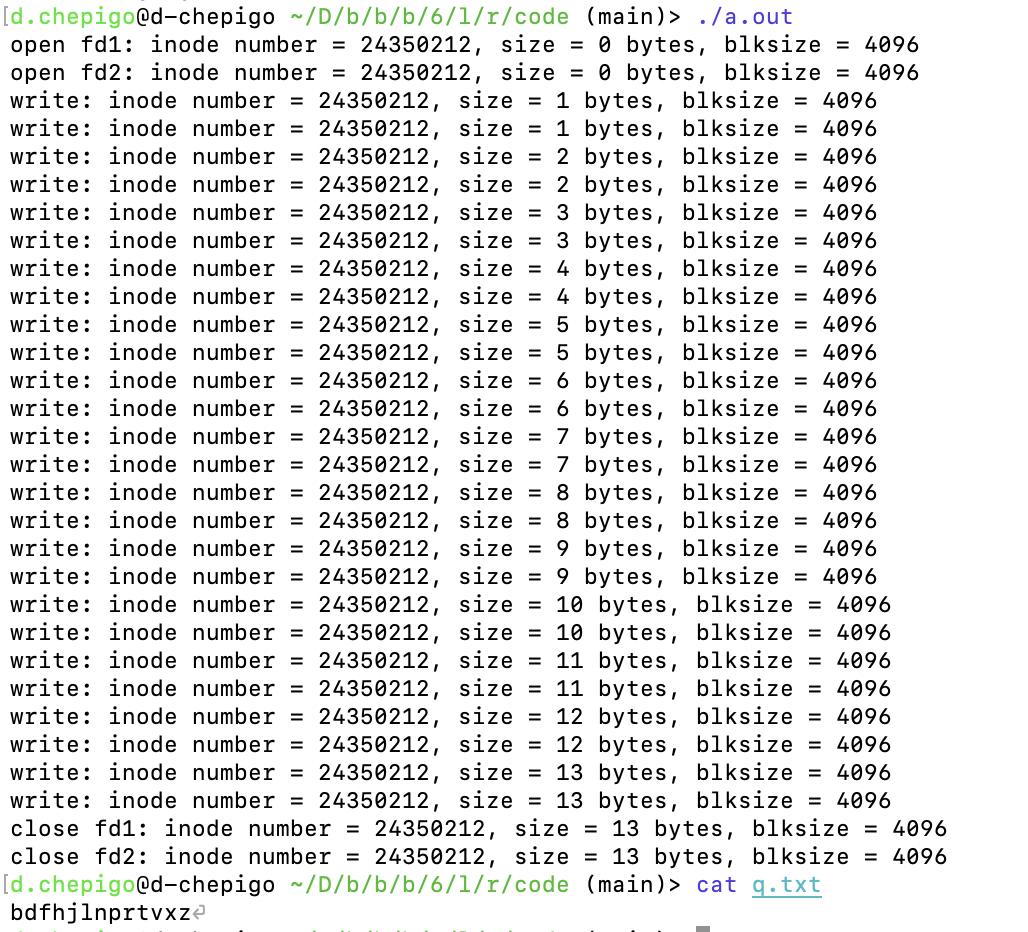
\includegraphics[width=\textwidth]{image/3-1}
	\caption{Вывод программы}
\end{figure}
В программе файл дважды открывается на запись функцией open(). В системной таблице открытых файлов создаётся два дескриптора struct file, каждый из которых имеет собственный указатель f\_pos, но оба ссылаются на один и тот же inode. С помощью системного вызова write() выполняется небуферизованный вывод. При изменении порядка вызова функций close() вывод программы не изменяется, так как вывод не буферизуется.

Чтобы вывести алфавит полностью, можно для второго открытия файла использовать open() с флагом O\_APPEND. В таком случае перед каждым вызовом write() для fd2 указатель f\_pos будет устанавливаться в конце файла, как если бы использовался lseek().

\newpage
\subsection{Связи структур}

\begin{figure}[!h!]
	\centering
	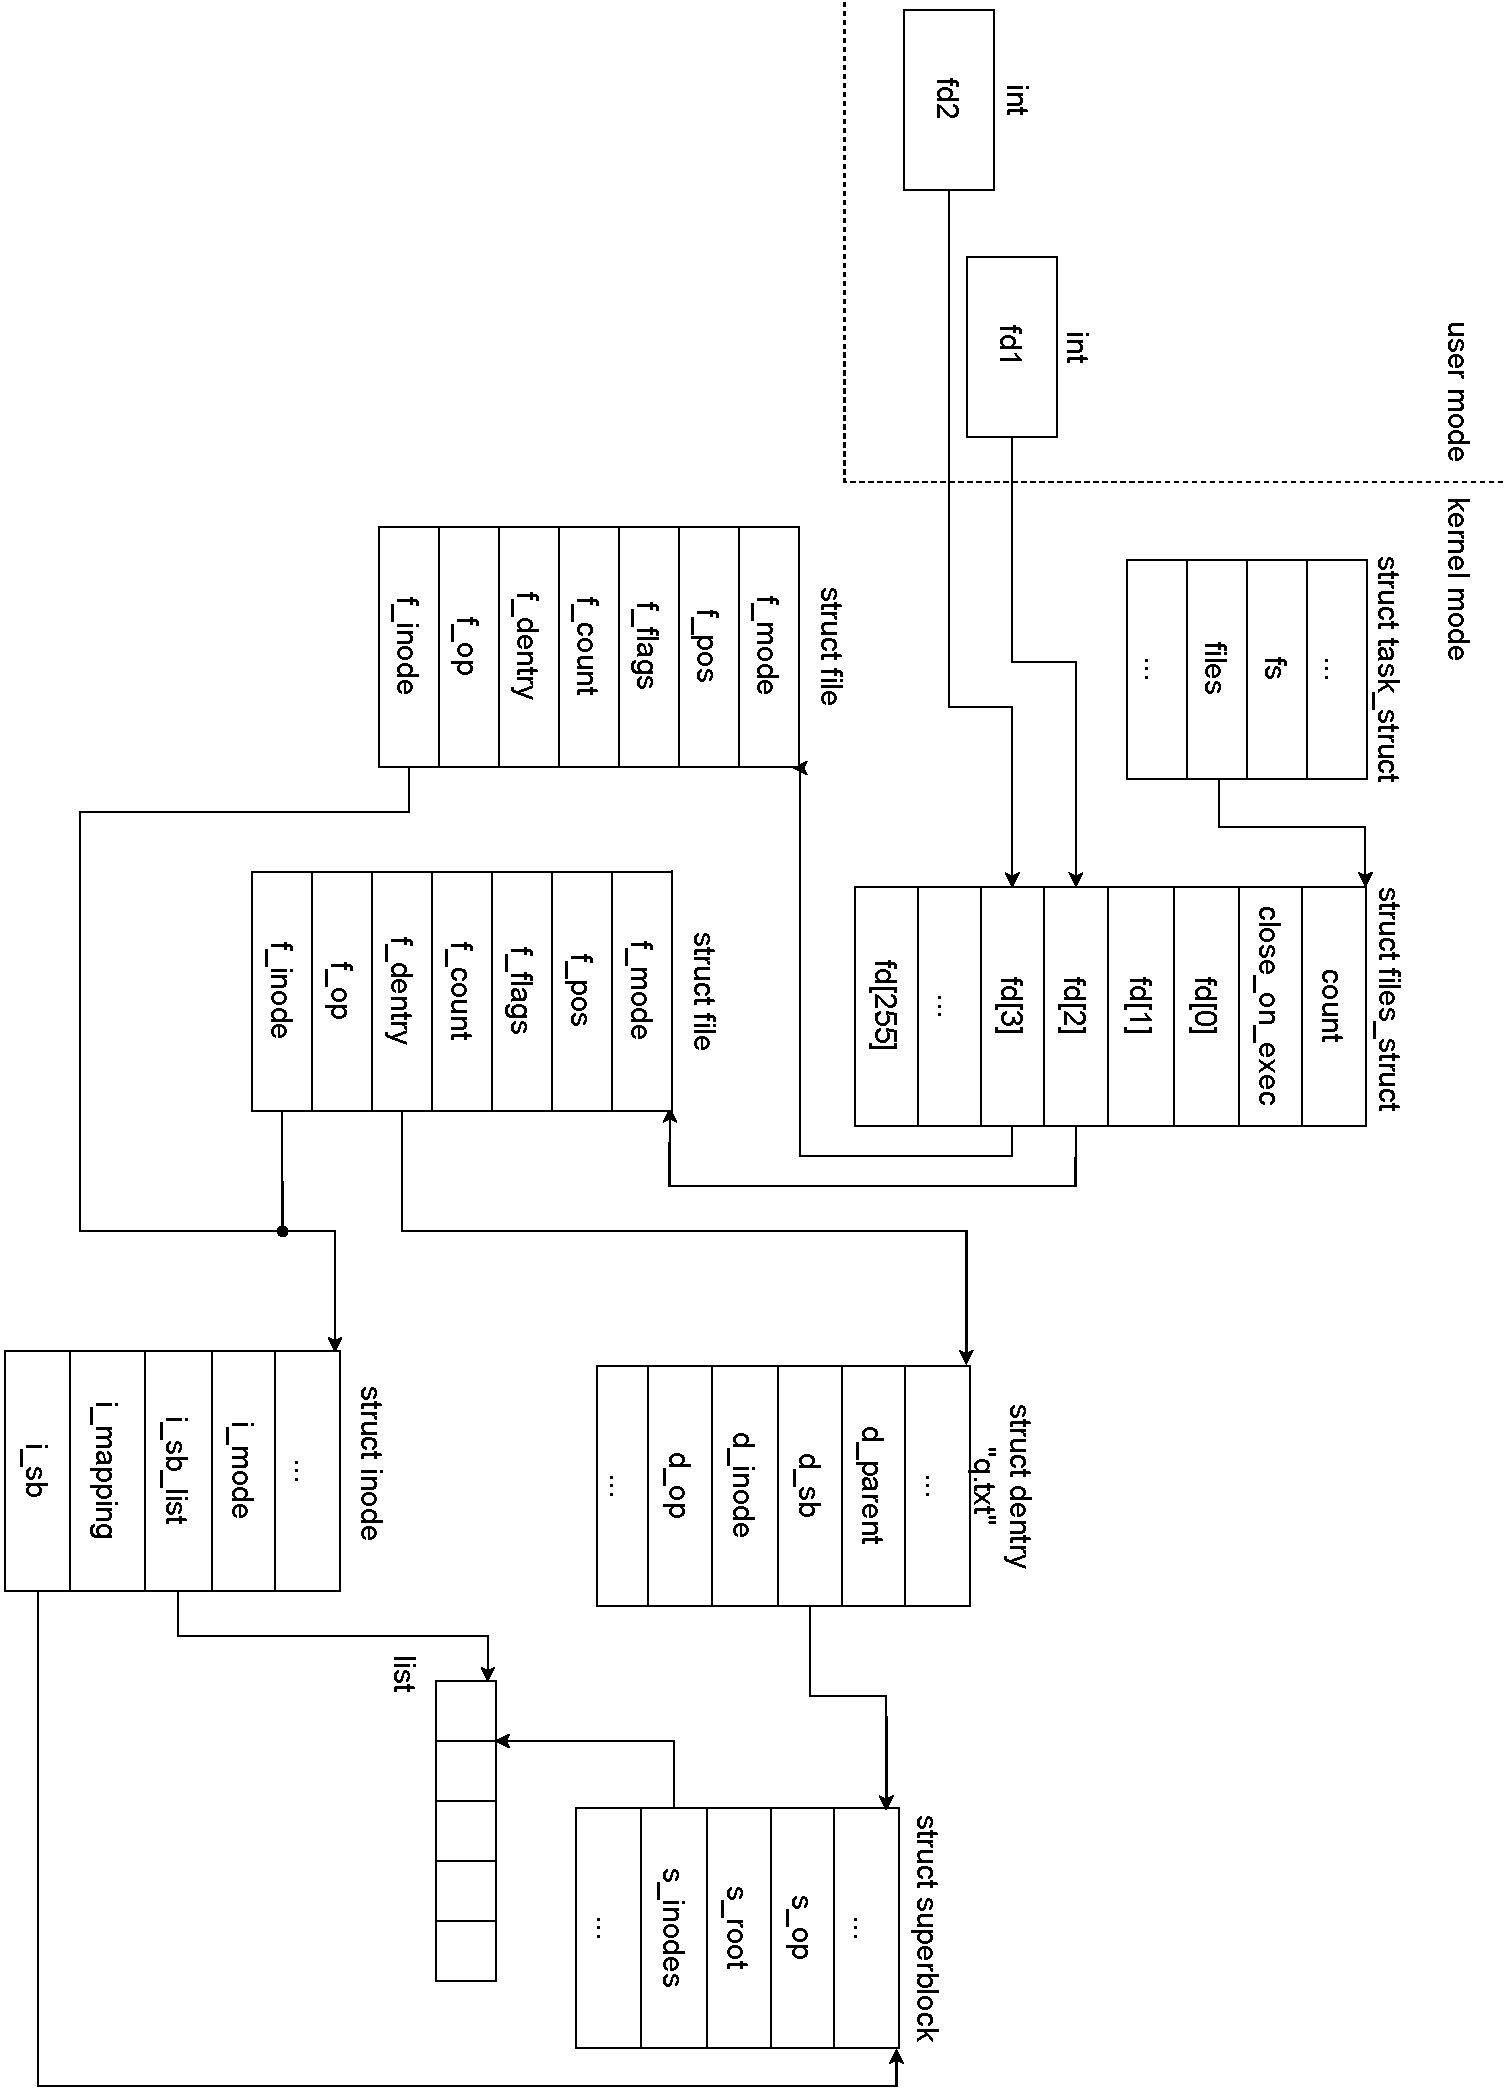
\includegraphics[width=150mm]{image/d4}
	\caption{Связи структур в третьей программе}
\end{figure}

\clearpage


\subsection{Многопоточный вариант}
\begin{code}
	\captionof{listing}{Третья программа с созданием двух дополнительных потоков}
	\inputminted
	[
	frame=single,
	framerule=0.5pt,
	framesep=10pt,
	fontsize=\small,
	tabsize=4,
	linenos,
	numbersep=5pt,
	xleftmargin=10pt,
	]
	{c}
	{code/3_2.c}
\end{code}
\newpage

\begin{figure}[!h]
	\centering
	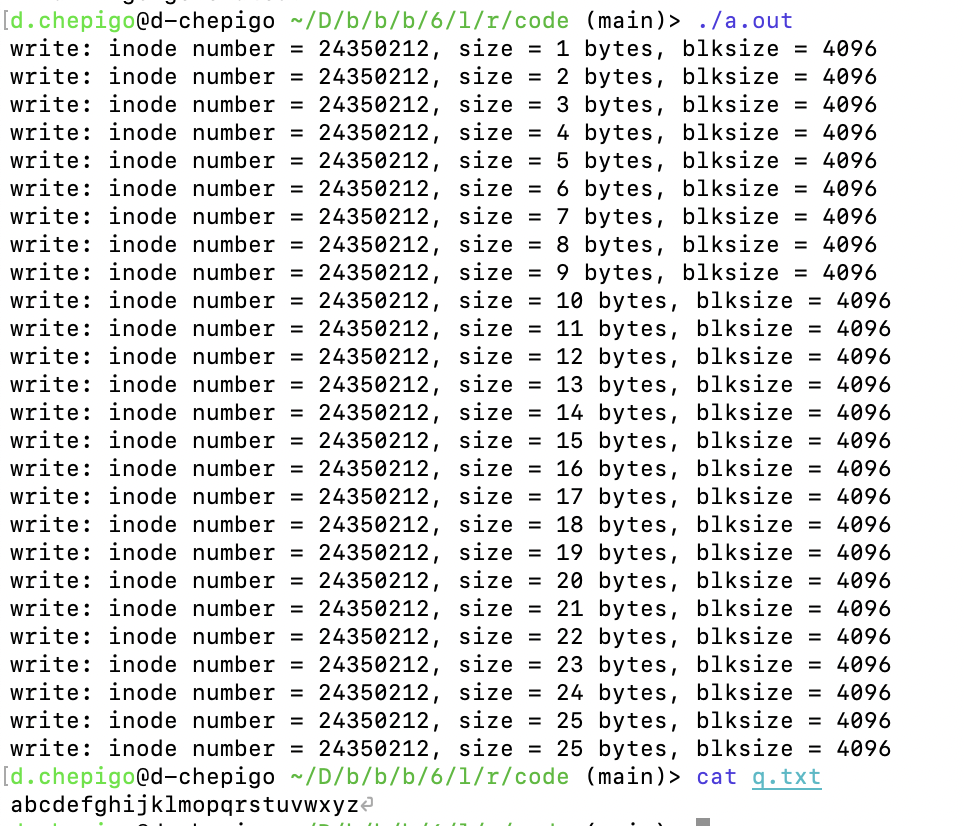
\includegraphics[width=\textwidth]{image/3-2}
	\caption{Вывод программы}
\end{figure}

В многопоточной программе работа с файлом производится аналогично однопоточной программе. Если не использовать средства взаимоисключения (например, мьютекс), то вторая половина алфавита будет записываться частично, и поведение программы будет не определено.

При создании дополнительных потоков связи структур не изменяются, так как ресурсами (в том числе и открытыми файлами) владеет процесс.

